\documentclass[../main.tex]{subfiles}

\begin{document}

    \Acrfullpl{kpi} are an important instrument to measure the outcome.
    In this section, I describe relevant \acrshortpl{kpi} for software development and incident management and how they are affected by the deployment workflow.
    To effectively prove an improvement over an existing process, representative data from a model running in the industry today would be required as a basis for further evaluation.

    I use cost as an indicator for success as it is one of the main drivers for the adoption of \gls{cloud_computing} by enterprises\cite{hc_patterns}.
    In a technical or mathematical model, time is usually the preferred unit of measurement.
    Time, however, is not a very reliable source for value unless there is a known, constant value for one unit of time.
    Cost on the other hand is universally understood and in most cases encapsulates time.
    Looking at it from a business perspective, the \acrlong{tco} has to be lower than the company income to generate profit.

    The metrics and formulas for software development and incident management outlined below, exemplify what the \acrlongpl{kpi} are, how they can be calculated and how the deployment process performance is a relevant factor.

    \subsubsection{Software development}

    Half of all large \acrshort{it} projects are estimated to overrun in both budget and time while at the same time delivering less value than expected.
    On top of that, the cost overruns increase with every year a project is running.
    The worst projects even cause bankruptcy.\cite{projects_overrun}

    To calculate the cost of a change, a few metrics are described and used to come up with a formula for software development cost that relates to deployments.

    \textbf{Lead time}
    is the time it takes to complete a change request, from the time it is taken up as a requirement to the moment when it is available in production.
    Lead time performance can vary greatly.
    While the elite has a lead time of less than a day, it takes between one and six months for low performers.\cite{four_key_metrics,state_of_devops_19}

    \textbf{Deployment lead time}
    is the time it takes for a commit to hit production.
    A quick deployment lead time enables developers to work more efficiently.\cite{devops_handbook_1}.

    \textbf{Deployment frequency}
    is an indicator for how often deployments are executed.
    An efficient deployment process is prerequisite for high frequency deployments.
    Values from the industry show similar performance differences as for lead time.\cite{four_key_metrics,state_of_devops_19}

    \textbf{Change failure rate}
    is the rate of changes that cause problems when deployed.
    Ideally, the change failure rate is zero.
    However, values up to 60\% have been reported in the industry.\cite{four_key_metrics,state_of_devops_19}

    Deployment cost includes everything that it takes to promote a change from commit to production, including all the hardware and computing cost for testing and releasing~\eqref{eq:deployment_cost}.
    Development cost is effectively the salary of the people required to perform a change~\eqref{eq:development_cost}.
    Change cost consists of the cost of development and the cost of deployment.
    The deployment cost grows linearly with the rate of failures to deliver a working solution~\eqref{eq:change_cost}.

    \subfile{concepts-eq-cost-dev}

    An automated, fast, easy-to-use deployment pipeline can have a positive effect on the deployment cost and therefore on the overall change cost.
    The benefit increases if a developer has to spend less time performing manual tasks.

    \subsubsection{Incident management}

    Based on industry surveys, the cost of an hour of outage is estimated well over USD 300 000.
    For large enterprises in the financial sector, this value can even go way above five million USD per hour.\cite{gartner_outage_cost,itic_outage_cost}

    Failures in the \gls{cloud} might be subject to \acrfullpl{sla} of the \gls{cloud} provider but that does not necessarily cover the damage of an outage and the potential breach of own \acrshortpl{sla}.
    The cost of downtime does not stop at revenue loss but also impacts reputation and hampers internal productivity.\cite{atlassian_cost_downtime}

    A company is responsible to have a backup plan for potential outages and design software to be resilient to failures.
    A key performance indicator for incident management is the \acrfull{mttr} a service.
    It is estimated to range from less than an hour to up to six months for the worst performers.
    \acrshort{mttr} can be further broken down into \acrlong{mttrc}, \acrlong{mttrp} and \acrlong{mttrs} (Fig.~\ref{fig:mttx_metrics}).\cite{state_of_devops_19}

    \begin{figure}[h]
        \centering
        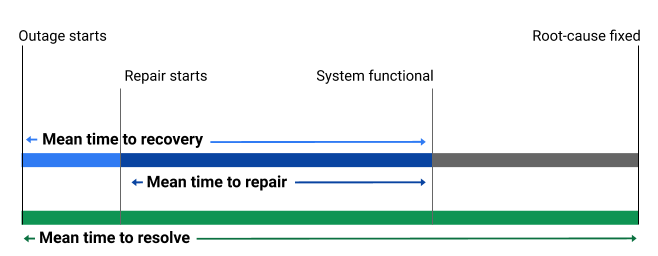
\includegraphics[width=0.95\linewidth]{img/concepts_eval_mttx_v2.png}
        \captionsetup{justification=centering}
        \caption{
            Overview of key performance metrics for incident management.\cite{atlassian_inc_metrics}
        }
        \label{fig:mttx_metrics}
    \end{figure}

    \textbf{\Acrfull{mttrc}}
    is the mean time between a failure of the system and the system being fully operational again.
    It reflects the effective outage time.\cite{atlassian_inc_metrics}

    \textbf{\Acrfull{mttrp}}
    is the mean time it actually takes to get the system operational again.
    Unlike \acrshort{mttrc}, this does not include the time it takes to find out what is causing the issue.\cite{atlassian_inc_metrics}

    \textbf{\Acrfull{mttrs}}
    covers the full cycle of resolving an issue.
    This includes fixing the root cause and preventing it from happening again.\cite{atlassian_inc_metrics}

    Recovery cost is the \acrlong{mttrc} multiplied by the average that an outage costs for the given time~\eqref{eq:recovery_cost}.
    The cost to fix the actual root cause is the remainder of the time it takes to resolve the problem multiplied by the average development cost~\eqref{eq:bug_fix_cost}.
    The sum of the recovery cost and the bug fix cost equals to the actual cost of an outage~\eqref{eq:outage_cost}.

    \subfile{concepts-eq-cost-inc}

    Both recovery cost and bug fix cost can be affected by the deployment process.
    A mechanism that allows to quickly redeploy failing applications into a different \gls{cloud} might help reduce \acrlong{mttrc} and therefore recovery cost significantly.

\end{document}